\section{Motivação}
Este trabalho foi motivado majoritariamente pela grande popularidade de integração e implantação contínuas, aliado a falta de estudos a este respeito no contexto da cidade de Recife.

\subsection{A grande adoção de CI e CD}
As práticas de integração e \emph{deployment} contínuos (\emph{Continuous Integration} e \emph{Continuous Deployment}) já são muito difundidas e utilizadas por empresas de tecnologia em todo o mundo. Segundo a pesquisa realizada pela empresa \emph{digital.ai} \cite{stateAgileReport2020}, 55\% dos participantes reportaram que sua organização pratica a técnica de integração contínua. Também nesta mesma pesquisa foi encontrado que 36\% utilizam a técnica de \emph{deployment} contínuos. 

Estes números elevados são causados principalmente pelos benefícios que a utilização destas técnicas trazem para a equipe e para o produto em desenvolvimento. Ainda de acordo com \cite{stateAgileReport2020}, entre as razões para adoção de CI/CD, as principais são aceleração de entregas de software (71\%), e aumentar a produtividade (51\%) e a qualidade do software (42\%). 

Especificamente sobre integração contínua, a prática hoje em dia já é bastante estudada difundida na indústria. O estudo \cite{hilton2016} comenta que desenvolvedores envolvidos se sentem mais produtivos quando utilizam a prática e dão mais valor aos testes automáticos.  Já com relação a \emph{deployment} contínuo, o estudo \cite{savor2015} mostra que seu uso traz maior qualidade ao software que está sendo produzido. 

\subsection{A falta de estudos no contexto Recifense}

Ainda há, no entanto, uma grande falta de estudos a respeito de como essas práticas foram importadas para a maioria das empresas \cite{empiricalStudy2016}, inclusive as de Recife, um dos grandes polos tecnológicos do Brasil. Somente no Porto Digital, localizado na capital pernambucana, há cerca de 330 empresas e 11 mil trabalhadores, com faturamento anual de R\$ 2,3 bilhões em 2019 \cite{portoDigital}.

O presente trabalho procura entender sobre a utilização das práticas de CI/CD nas empresas de Recife para que esses dados sirvam como objeto de pesquisa para levantamento de possíveis dores sentidas pelos desenvolvedores locais que justifiquem a adoção ou não destas práticas. Um estudo a respeito de como as técnicas de integração e \emph{deployment} contínuo migraram para a indústria de Recife funciona ainda como um \emph{benchmark} de como as empresas estão se portando em relação às novidades presentes na literatura nos últimos anos, assim como levantar possíveis discrepâncias entre empresas situadas na área e as grandes corporações. 


\subsection{O artigo base}
Com o objetivo de entender um pouco mais sobre o estado da prática de CI/CD no contexto de Recife, nos baseamos no estudo \cite{empiricalStudy2016}, que busca entender como as práticas geralmente associadas a \emph{Continuous Deployment} acharam o seu caminho nas indústrias européia e norte-americana. Nesse estudo os autores utilizaram um método misto de estudo empírico baseado em um pré-estudo na literatura, entrevistas com 20 participantes e um \emph{survey} que recebeu 187 respostas. A ideia era questionar até que ponto o conhecimento na área estava dominado por peculiaridades de um pequeno grupo de grandes empresas, como Facebook e Google.

Os autores também definem a chamada \emph{stairway to heaven} (escada para o céu, em tradução livre), presente na Figura \ref{stairway}. Ela tem como objetivo definir um caminho de evolução das empresas para um estágio de entregas sofisticado. A escada permeia práticas de integração contínua, \emph{deployment} contínuo e entregas parciais.

\begin{figure*}
% \begin{center}
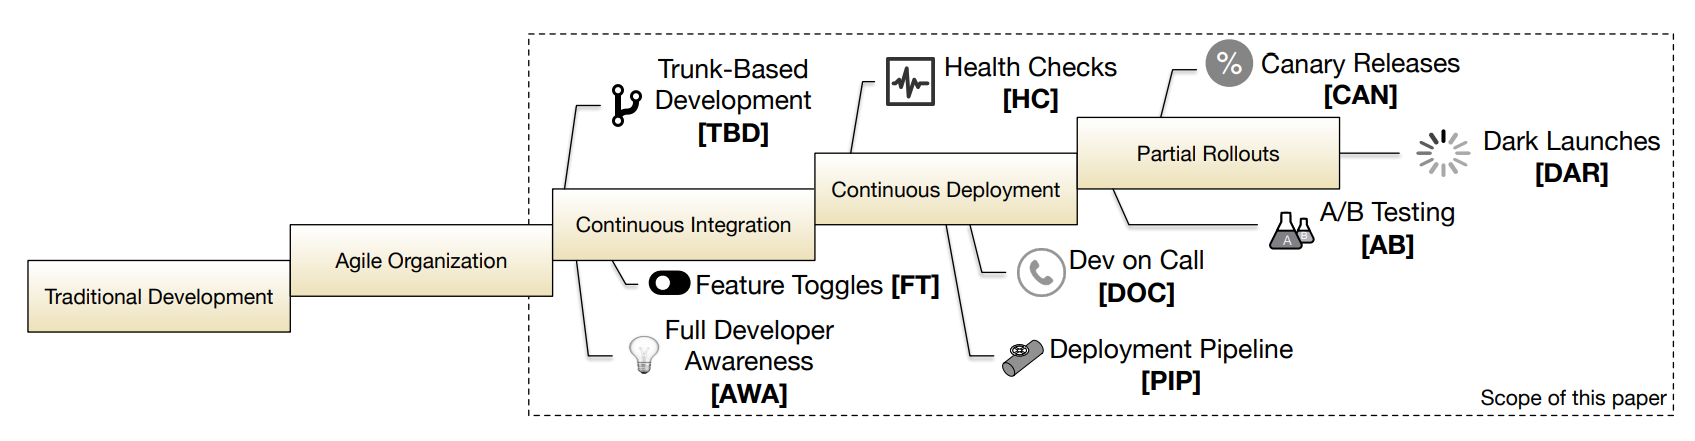
\includegraphics[width=\textwidth]{stairway_to_heaven.png}
% \end{center}
\caption[Stairway to Heaven]{
    A escada de evolução denominada \emph{Stairway to Heaven} proposta pelo artigo base.
    Fonte: Schermman et al \cite{empiricalStudy2016}
}\label{stairway}

\end{figure*}

Através desta metodologia os autores descobriram que, no contexto estudado, problemas arquiteturais são geralmente uma das maiores barreiras para a adoção de CD. Não obstante, a técnica de \emph{Feature Toggles} \cite{featureToggles} como forma de realizar entregas parciais adiciona uma complexidade demasiada e não saudável ao código. Por fim, eles concluem que os desenvolvedores necessitam também de um protocolo baseado em princípios que estabeleçam quando deve-se utilizar técnicas de entregas parciais, por exemplo, que funcionalidades e métricas devem ser testadas por um teste A/B \cite{testsAB}.

Aprender mais sobre as dificuldades que outras empresas não globais sofrem no processo de adoção de práticas de CI/CD pode gerar mais estudos a respeito de como solucionar tais problemas, assim como mostrar possíveis oportunidades de melhoria e revisão dos processos utilizados. Um trabalho que utilize uma adaptação da metodologia aplicada a uma amostra de um outro contexto pode revelar ainda discrepâncias e semelhanças entre os dois ambientes de estudo. As discrepâncias levantariam pontos de questionamento, pesquisa e até possíveis melhorias aos ambientes envolvidos. Já as semelhanças podem assegurar que as práticas utilizadas já acharam o seu lugar na indústria e funcionam bem assim como a teoria propunha.

Assim, a grande adoção da indústria mundial das práticas de CI/CD, aliado a falta de trabalhos a respeito no contexto recifense, além da metodologia já validada proposta pelo artigo foram as principais motivações para o desenvolvimento deste trabalho

\subsection{Perguntas de pesquisa} 
Com o intuito de entender como as técnicas de integração, entrega e \emph{deployment} contínuos foram importadas para as empresas recifenses, as seguintes perguntas de pesquisa foram formadas:

\begin{enumerate}
\item Quais as práticas de CI/CD são utilizadas pelas empresas em Recife?
\item O cenário de CI/CD nas empresas em Recife segue o \emph{stairway to heaven} proposto no artigo?
\item Quais são os princípios e práticas subjacentes que governam a adoção de CI/CD na indústria?
\end{enumerate}

Para responder às perguntas acima foi decidido aplicar a pesquisa qualitativa do artigo \cite{empiricalStudy2016} com desenvolvedores recifenses, baseando-se também na mesma lista de definições de cada uma das práticas envolvidas no \emph{Stairway to Heaven}. A pesquisa qualitativa neste contexto foi considerada fundamental para garantir que os entrevistados entendessem claramente as perguntas e excluir possíveis entendimentos errados de termos em inglês, linguagem não nativa de todos os participantes. Vale salientar que não foi replicado a pesquisa quantitativa presente no artigo base devido à falta de tempo hábil para tal, mas esta pode servir como um trabalho futuro a este.

Além disso, as perguntas 1 e 3 são uma adaptação das perguntas 1 e 2 do artigo base \cite{empiricalStudy2016}, respectivamente, incluindo a técnica de \emph{Continuous Integration}. Não obstante, uma terceira pergunta foi adicionada (\emph{RQ2}), que foca na escada de evolução proposta pelo artigo. Ela tenta responder se a \emph{stairway to heaven} é seguida no contexto de Recife, visto que, no outro, os próprios autores já refutaram esta definição com os seus resultados.
